\documentclass[notitlepage]{article}
\usepackage[T1, T2A]{fontenc}
\usepackage[utf8]{inputenc}
\usepackage[russian]{babel}
%
%\usepackage{newtxmath}
%\usepackage {fouriernc} %bold
%\usepackage{kpfonts}
%%
%\usepackage{gentium}
%\usepackage[default]{droidserif}
%\usepackage{XCharter} %bold
%
\usepackage{import}
\usepackage{mathtools}
\usepackage{bm}
\usepackage{tikz, enumerate, graphicx, amsmath, amssymb, amsthm}
\let\epsilon\varepsilon
\DeclareMathOperator{\conv}{Conv}
\DeclareMathOperator{\expect}{\mathbb{E}}
\DeclareMathOperator{\res}{Res}
\DeclareMathOperator*{\argmax}{arg\,max}
\DeclareMathOperator{\N}{\mathcal{N}}
\DeclareMathOperator{\KL}{KL}
\DeclareMathOperator{\cov}{cov}
\DeclareMathOperator{\const}{const}
\DeclareMathOperator{\cat}{Cat}
\DeclareMathOperator{\diag}{diag}

%\usepackage[paperwidth=13.33in,paperheight=7.5in,margin=1in,heightrounded]{geometry}
\title{Проект по курсу ``Эффективные модели ML и архитектуры нейросетей''}
\author{Иван Ермаков\\
        М05-314а}
\date{}
\begin{document}
\maketitle
\section{Introduction}
В настоящее время нейросетевые модели являются передним краем науки (State-of-the-Art) в подавляющем большинстве задач машинного обучения.
Примерами могут быть задачи компьютерного зрения, обработки естественного языка и обучения на табличных данных.
Одним из важнейших преимуществ нейронных сетей является избавление от эвристик, присущих классическим алгоритмам обучения.
Это способствует большей предсказательной силе нейросетевых моделей при условии применения достаточного числа данных.
Однако большим минусом нейросетевых моделей является большая сложность обучения и связанная с этим неопределенность в выборе так называемых \textit{гиперпараметров}, которые значительно влияют на качество полученной модели.
В настоящее время наиболее распространённым способом для оптимизации гиперпараметров является ручной подбор~\cite{bouthillier2020survey}.
Однако из-за больших трудозатрат этот подход нельзя признать удовлетворительным.

В силу того, что гиперпараметры имеют совершенно разный характер, многие из них не допускают дифференцирование выхода сети, либо такие алгоритмы не реализованы, к оптимизации гиперпараметров приходится подходить как к ``чёрному ящику'' (\textit{black-box optimization}).
Это исключает градиентные и даже выпуклые методы для оптимизации, оставшиеся же заметно уступают в скорости.
Именно скорость является главной проблемой: один сеанс обучения нейросети может занимать часы, а запусков могут потребоваться десятки.
Поэтому большой интерес представляют методы для ускорения подбора гиперпараметров.

Одним из подходов здесь является ранняя остановка безперспективных исследований.
Для этого используются какие-либо промежуточные результаты.
Один из подходов к такой остановке предложен в данной работе.
\section{Обзор}
Оптимизация гиперпараметров --- это обширная тема, и ей посвящено большое количество обзоров, например~\cite{yu2020hyper}.

Оценка похожести нейронных сетей осуществляется обычно исходя из выходов нейросети (не весов).
Если есть выходы $X \in \mathbb{R}^{m\times n}$ и $Y \in \mathbb{R}^{k\times t}$ разных слоёв одной и той же, либо разных моделей, то для определения их схожести есть следующие методы:
\begin{itemize}
    \item Линейная регрессия между $X$ и $Y$ --- коэффициентов является $R^2$
    \item CCA~\cite{ramsay1984matrix}. Находятся базисы, после проекции $X$ и $Y$ на которые корреляция максимизируется.
    \item SVCCA~\cite{golub1995canonical}. То же самое, но после SVD-разложения.
    \item Projection-Weighted CCA~\cite{morcos2018insights}
    \item Mutual information
    \item CKA~\cite{kornblith2019similarity}
\end{itemize}

CKA является широко принятым методом, поэтому я буду использовать его, в его линейном варианте.
За дальнейшими деталями отсылаю к оригинальной работе.
\section{Методы}
Для оценки качества обучения нейросети будем использовать коэффициент корреляции CKA~\cite{kornblith2019similarity}.
Сам по себе он непригоден для этого, однако ещё в оригинальной работе содержится идея, что у плохо обученных нейросетей
корреляция между выходами промежуточных слоёв и выходом последнего слоя велики: нейросеть не использует последние слои эффективно, что может говорить
о проблемах с обучением.
Поэтому определим для обученной нейронной сети из $n$ слоёв $W_i(x)$ ($i$ --- номер слоя) коэффициент $\textit{CKA}$:
\begin{equation}
    CKA(W, X) = \sum_{i = 1}^{n - 1} \mathrm{cka}\,(W_i(X), W_n(X))
\end{equation}
На основе этого значения и будем производить остановку экспериментов.
\section{Эксперименты}
\subsection*{Экспериментальный пайплайн}
Для исследования принципиальной возможности ускорения подбора гиперпараметров была использована задача классификации изображений на датасете CIFAR-10~\cite{krizhevsky2009learning}.
Нейросеть представляет из себя 2 свёрточных и 2 полносвязных слоя с \verb|MaxPool2d| и активациями \verb|ReLU|.
\begin{figure}[ht]
    \centering
    \includegraphics*[width=\linewidth]{imgs/net.png}
    \caption{Архитектура использованной нейронной сети}
\end{figure}
В качестве целевого лосса стандартно выбрана кросс-энтропия, оптимизация с использованием оптимизатора Adam.
В качестве гиперпараметров были выбраны:
\begin{itemize}
    \item Learning rate
    \item Количество эпох
    \item Label smoothing в кросс-энтропийном лоссе
    \item Weight Decay для Adam
\end{itemize}

Для оптимизации гиперпараметров был использован один из широко распространённых фреймворков Optuna~\cite{optuna_2019}.
Используемый метод --- Tree-structured Parzen Estimator~\cite{bergstra2011algorithms}.
Замечу, однако, что конкретный метод семплирования не имеет значения для данной работы.
Области поиска параметров представлены на таблице~\ref{tab:hyp}.
\begin{table}[ht]
    \begin{tabular}{llll}
    Параметр        & Тип   & Левая граница & Правая граница \\ \hline
    Learning Rate   & float & $10^{-4}$     & $10^{-2}$      \\ \hline
    Weight Decay    & float & $0$           & $10^{-3}$      \\ \hline
    Label Smoothing & float & $0$           & $1$            \\ \hline
    \#epochs        & int   & 5             & 20
    \end{tabular}
    \caption{Области значений гиперпараметров}
    \label{tab:hyp}
\end{table}
Дополнительно для Learning Rate было выбрано лог-равномерное распределение, чтобы точнее отразить влияние этого параметра.
Бюджет для исследования --- 100 обучений.
В ходе каждого эксперимента сеть обучалась с выбранными значениями гиперпараметров и после каждой эпохи значения показателя CKA сохранялись.
Сама оптимизация гиперпараметров происходила при помощи оценки точности на валидационной части датасета.
Показатель CKA при этом считался по выходам двух свёрточных и двух полносвязных слоёв на одном батче валидационной выборки.

Для исследования предлагается простейшая техника отсечения испытания по порогу метрики \textit{CKA}: заранее выбирается порог и если через заданное число $k$ эпох \textit{CKA}
оказывается больше порога, то дальше обучение не продолжается.

\subsection*{Результаты}
На рисунке~\ref{fig:result} приведены графики корреляции \textit{CKA} и итоговой точности на валидационной части датасета в зависимости от числа эпох $k$ перед отсечением.
\begin{figure}[ht]
  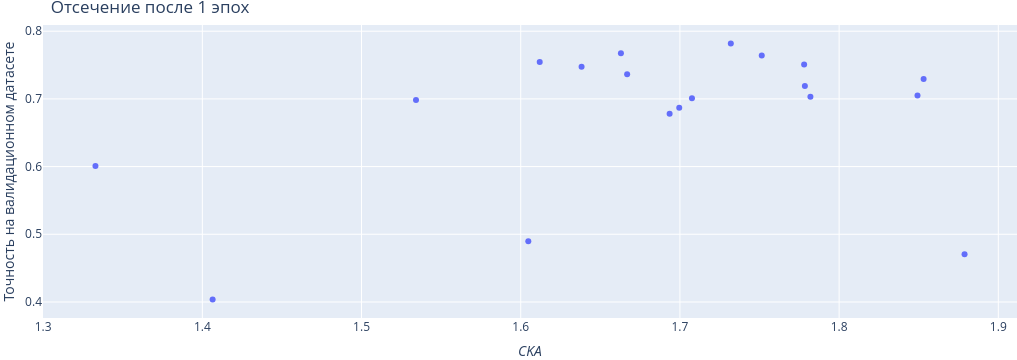
\includegraphics[width=\linewidth]{imgs/1_epochs.png}
  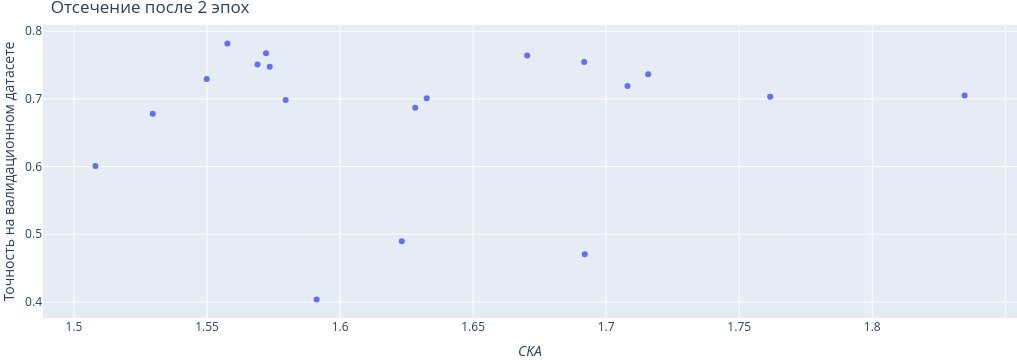
\includegraphics[width=\linewidth]{imgs/2_epochs.png}
  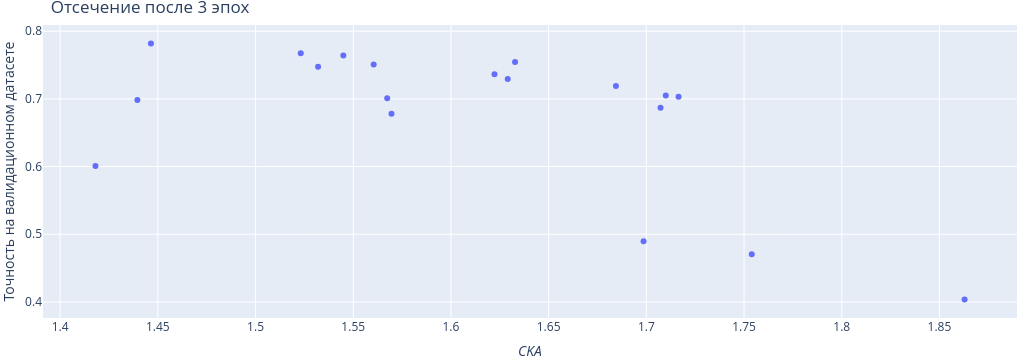
\includegraphics[width=\linewidth]{imgs/3_epochs.png}
  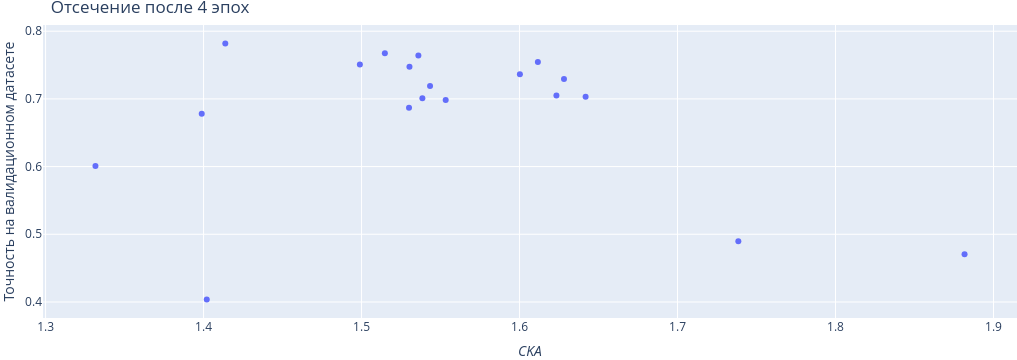
\includegraphics[width=\linewidth]{imgs/4_epochs.png}
  \label{fig:result}
  \caption{Результаты экспериментов}
\end{figure}
Несмотря на то, что подбор гиперпараметров может быть произведён на 100 эпохах, такой эксперимент закончился неудачей из-за технических сложностей, которые не было возможности вовремя устранить.
Тем не менее, он был проведён в сокращённом варианте на 19 испытаниях.

Можно заметить, что после первой эпохи, как и после второй, корреляция практически не просматривается.
Однако уже после третьей, а особенно после четвёртой, корреляция становится всё более чёткой.
Это позволяет выбрать порог, например, в $CKA = 1.5$, при достижении которого обучение можно прерывать.
Данная оптимизация позволит отсечь более 80\% испытаний после 4 эпохи, тем самым значительно сократив время исследования.

Также представляет интерес выбор порога для отсечения обучения после \textit{половины} эпох.
График для этого эксперимента представлен на рисунке
\begin{figure}[ht]
    \centering
    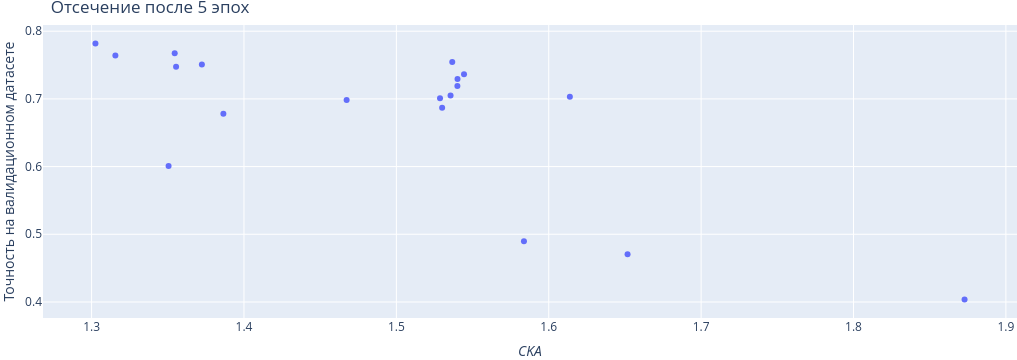
\includegraphics[width=\linewidth]{imgs/half_epochs.png}
    \caption{Отсечение после половины эпох}
\end{figure}
Очевидно, здесь также подходит порог $CKA = 1.5$.

\section{Выводы}
Предложенный подход к оптимизации подбора гиперпараметров нейронных сетей позволяет значительно ускорить этот длительный процесс.
Однако малое количество данных оставляет много вопросов, и, несомненно, одним из возможных дальнейших направлений для исследования может стать
проведение эксперимента с значительно большим числом испытаний.
Также интересна устойчивость метрики: насколько много ситуаций, когда мы отсечём лучшее испытание?
Кроме того, насколько вероятна ситуация, когда отсечено будет не просто лучшее испытание, но испытание, которое \textit{заметно} лучше оставшихся?
Наконец, стоит исследовать применимость других метрик схожести сетей, кроме CKA, и проверить предложенный метод в других областях машинного обучения.

\bibliographystyle{unsrt}
\bibliography{references}
\end{document}